\section{Rezultatai}

Sukurtas įrankis įgalina realiu laiku iš kartais nevisai gerai ir tiksliai
išsaugotų tūrinių duomenų išgauti akiai daug malonesnius vaizdinius.

Kaip funkcionalumo pavyzdį pateiksiu keturių turinių objektų išvaizdos
apdorojimą, pasiektą šiuo įrankiu.

Pirma, turime tiesioginę vokselių interpretaciją. Vokselių permatomumo
reikšmės tiesiogiai atvaizduojamos skalėje $0.0 \ldots 1.0$ (Pav.
\ref{fig:compare_0}). Tada objektams pritaikomas transformavimo filtras (Pav.
\ref{fig:compare_1}). Objektų išvaizda dar šiek tiek pakoreguojama globaliu
permatomumo filtru (Pav. \ref{fig:compare_2}). Galiausiai pritaikomas
apšvietimo sustiprinimo filtras ir gaunamas galutinis vaizdas (Pav.
\ref{fig:compare_3}).

Kaip jau minėta, įrankis nėra skirtas dideliam kiekiui, ar dideliam
vaizdavimo greičiui pasiekti -- tai kitų temų sritis. Tačiau, realaus laiko
savoka įpareigoja pateikti kadrų per sekundę rezultatus\footnote[1]{Naudota techninė įranga: Intel Pentium(R) 4 CPU 3.00GHz; 1 GB
RAM; NVIDIA GeForce 9500 GT (512 MB Ram). Vaizdavimo rezoliucija $846x464$.}

(Lentelė \ref{tab:fps}).

\begin{table}[!ht]
\centering
  \begin{tabular}{ | r | r | r | r | }
  \cline{1-4}
  Scenos padalijimas    &     $49x49x49$ &    $64x64x64$ & $98x34x34$   \\ \hline
  Kadrai per sekundę    &          96.01 &         93.54 &      90.24   \\ \hline
  Scenos padalijimas    &  $256x256x128$ & $256x256x256$ & $301x324x56$ \\ \hline
  Kadrai per sekundę    &          59.21 &         59.24 &        50.28 \\ \hline
  \end{tabular}
\caption{Kadrai per sekundę (vidurkis), vaizduojant įvairių dydžių tūrinius objektus. }
\label{tab:fps}
\end{table}

\begin{figure}[b]
\centering
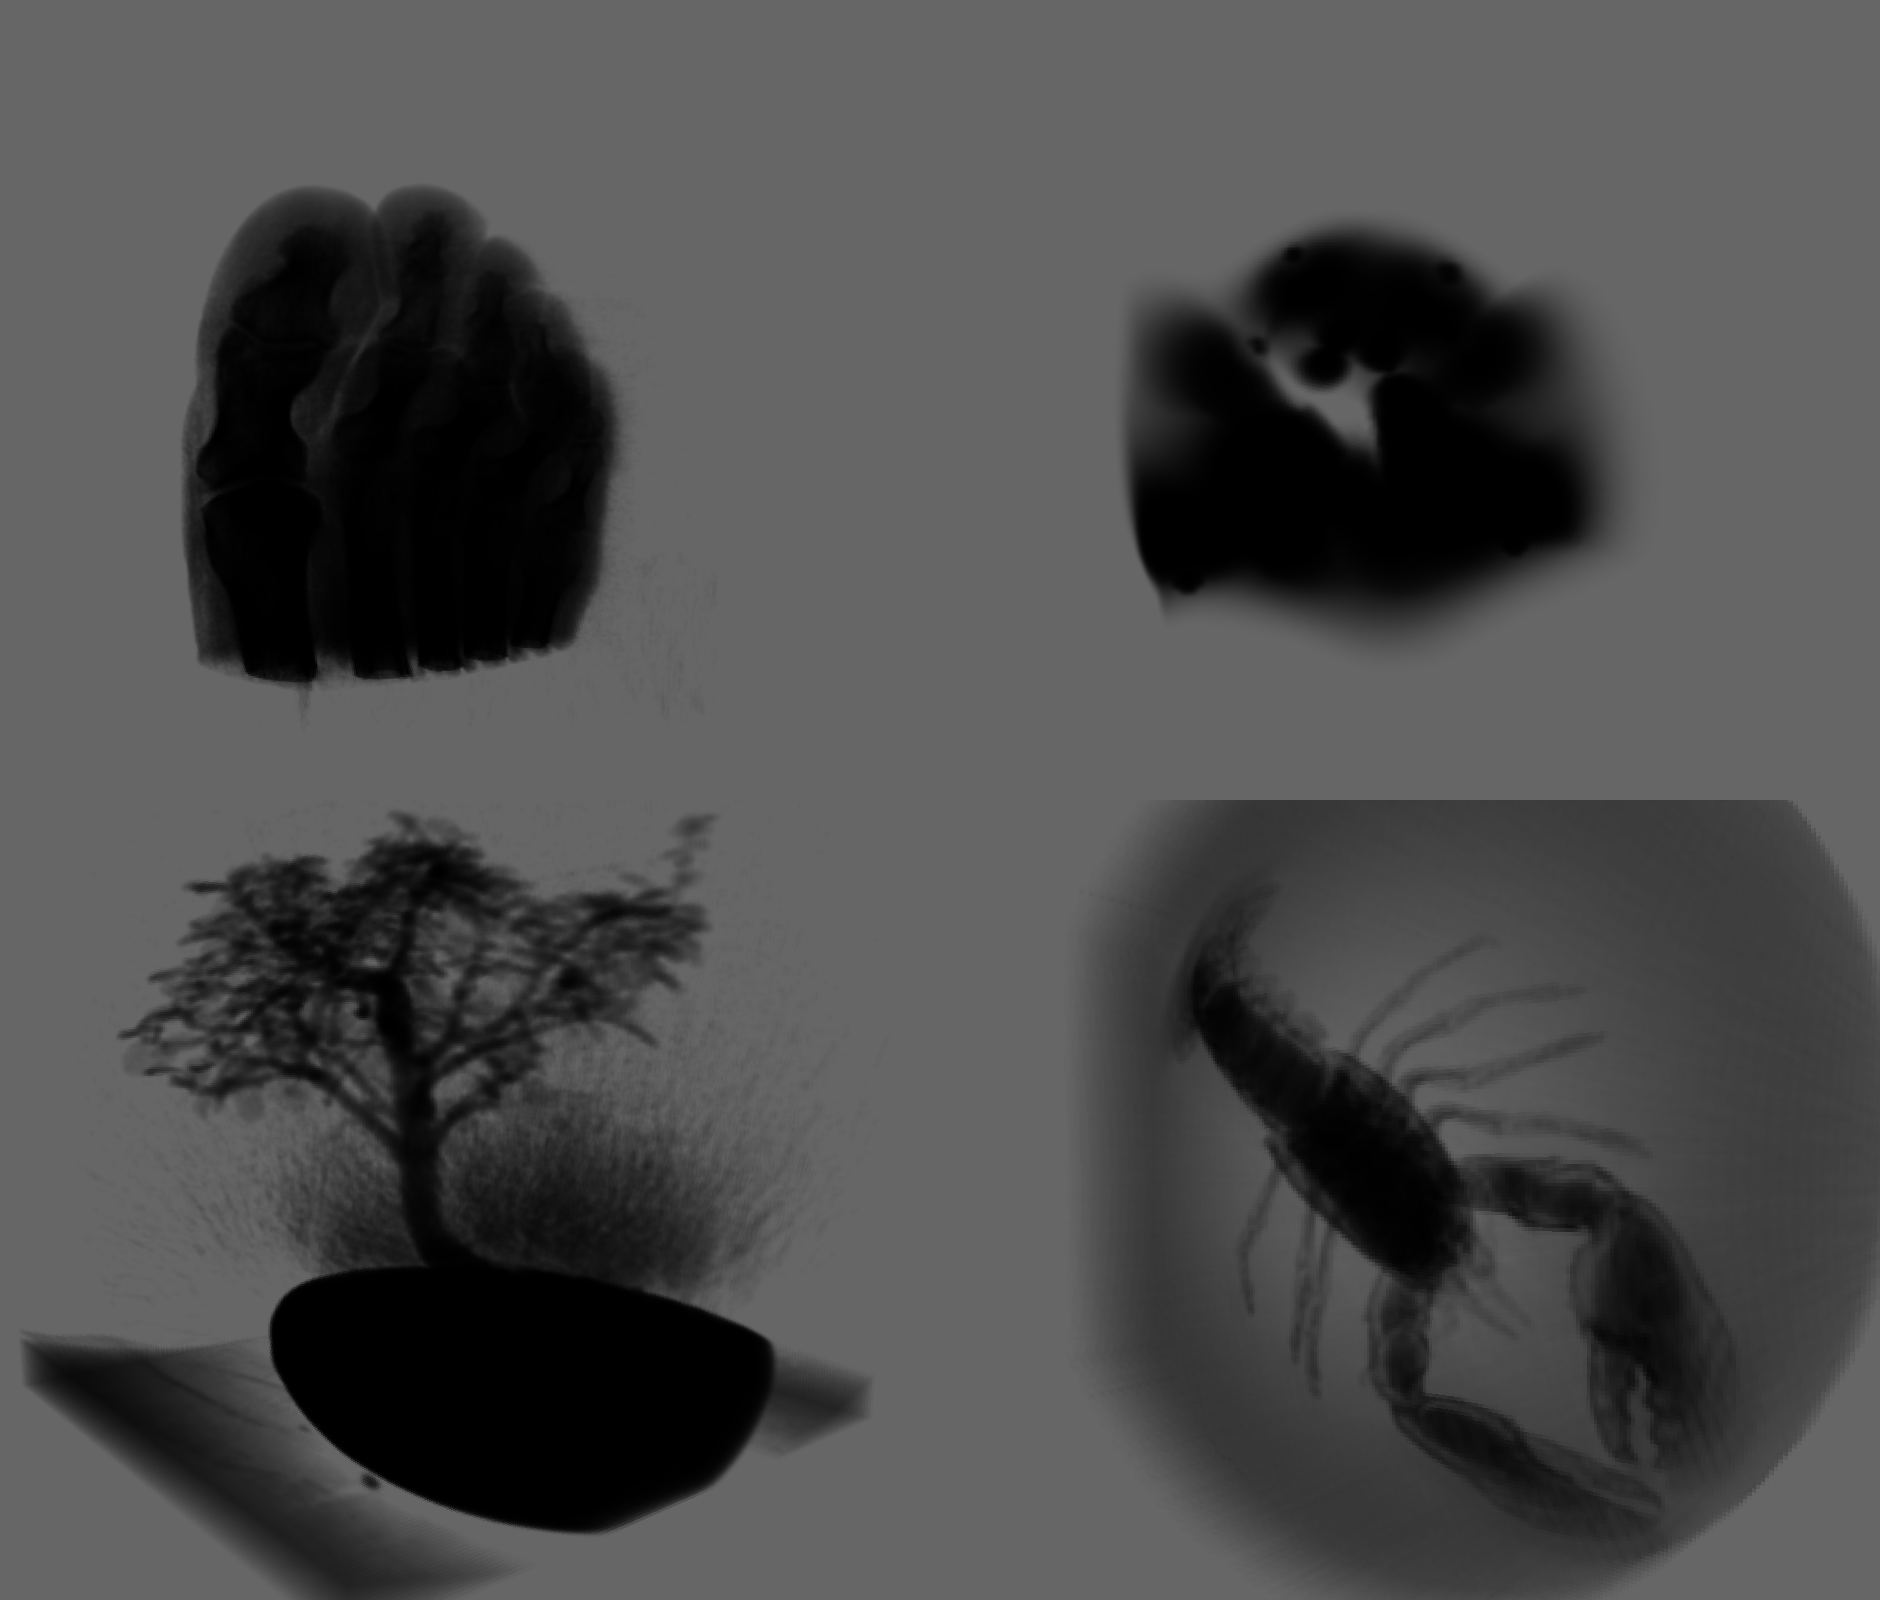
\includegraphics[height=11.5cm]{compare_0.png}
\caption{Pradinės tūrinių objektų vizualizacijos.}
\label{fig:compare_0}
\end{figure}

\begin{figure}[b]
\centering
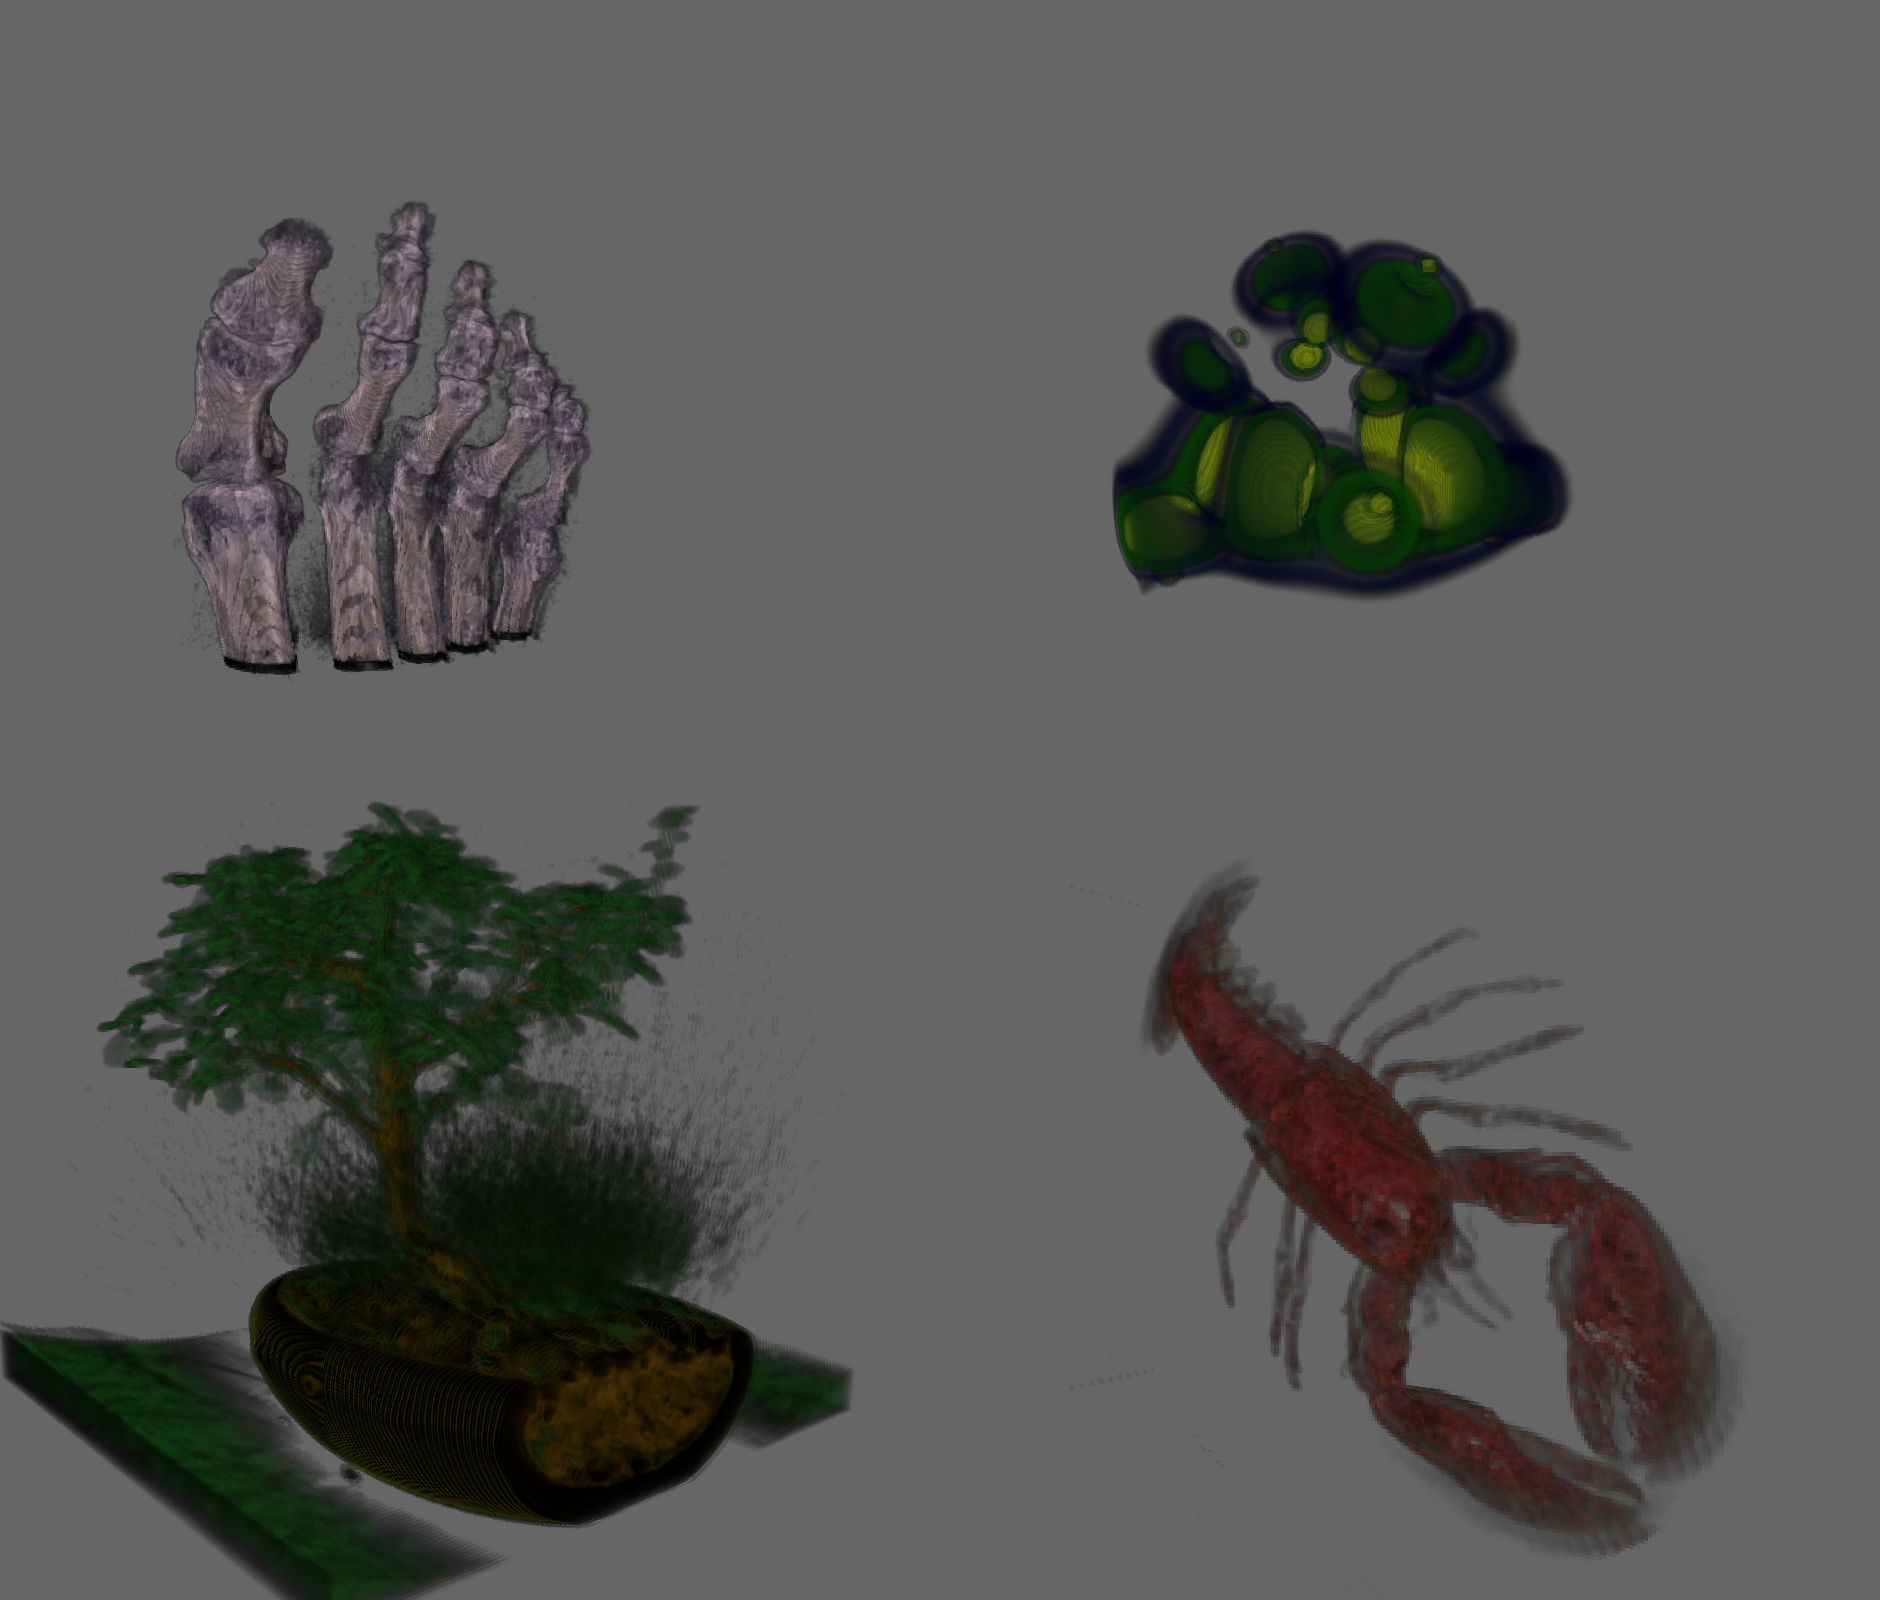
\includegraphics[height=11.5cm]{compare_1.png}
\caption{Transformavimo filtras.}
\label{fig:compare_1}
\end{figure}

\begin{figure}[b]
\centering
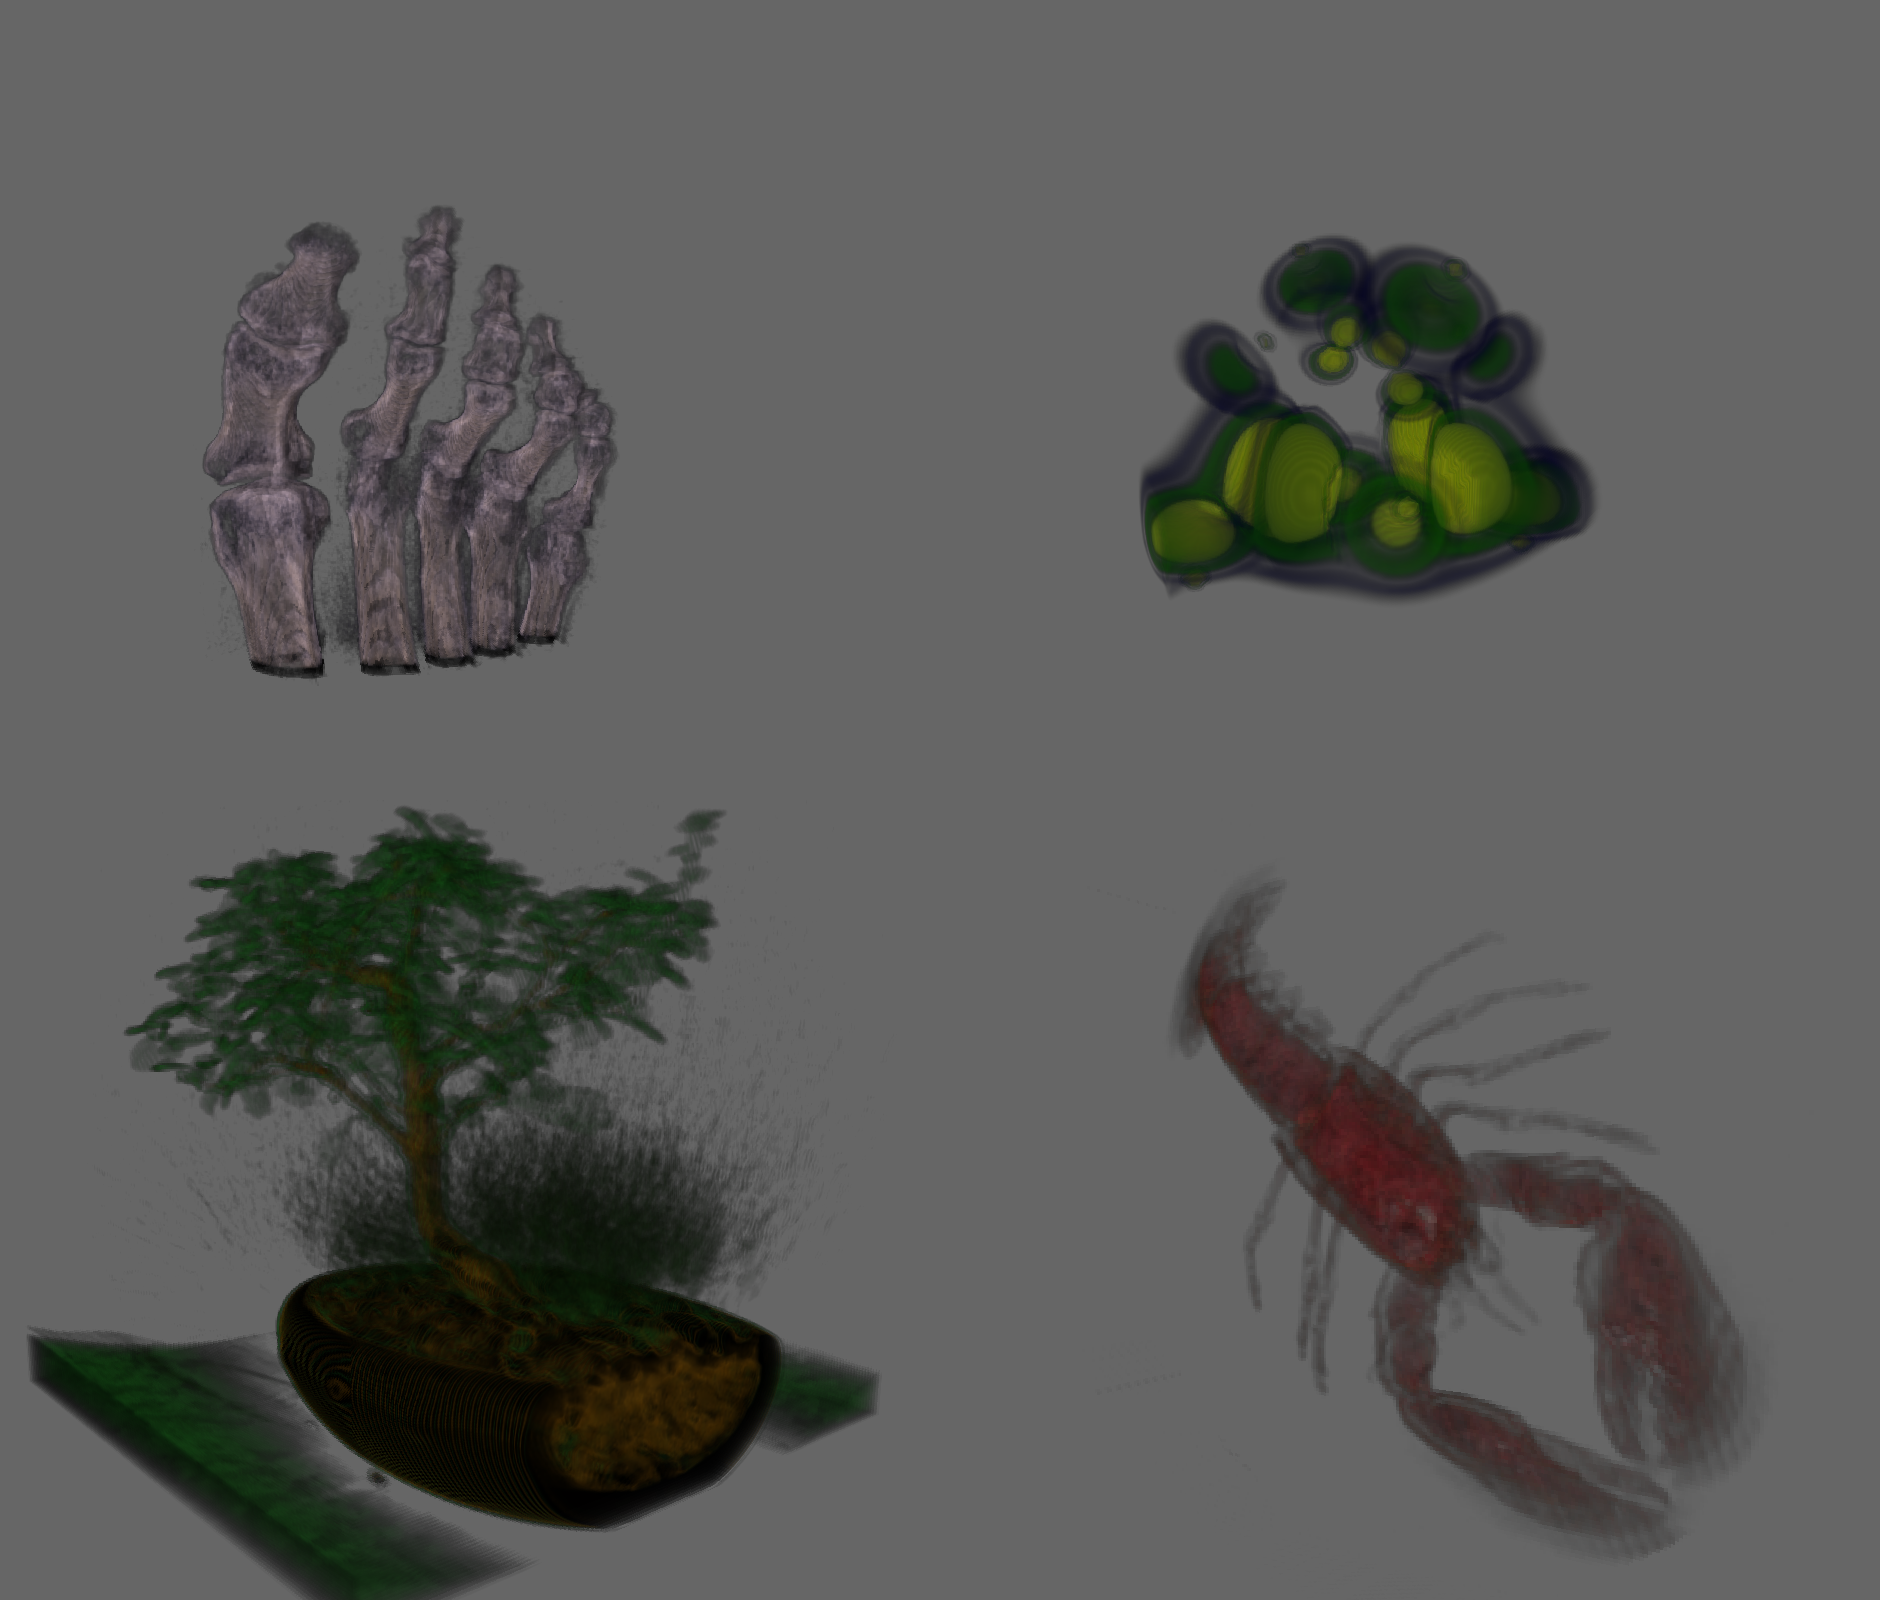
\includegraphics[height=11.5cm]{compare_2.png}
\caption{Globalaus permatomumo filtras.}
\label{fig:compare_2}
\end{figure}

\begin{figure}[b]
\centering
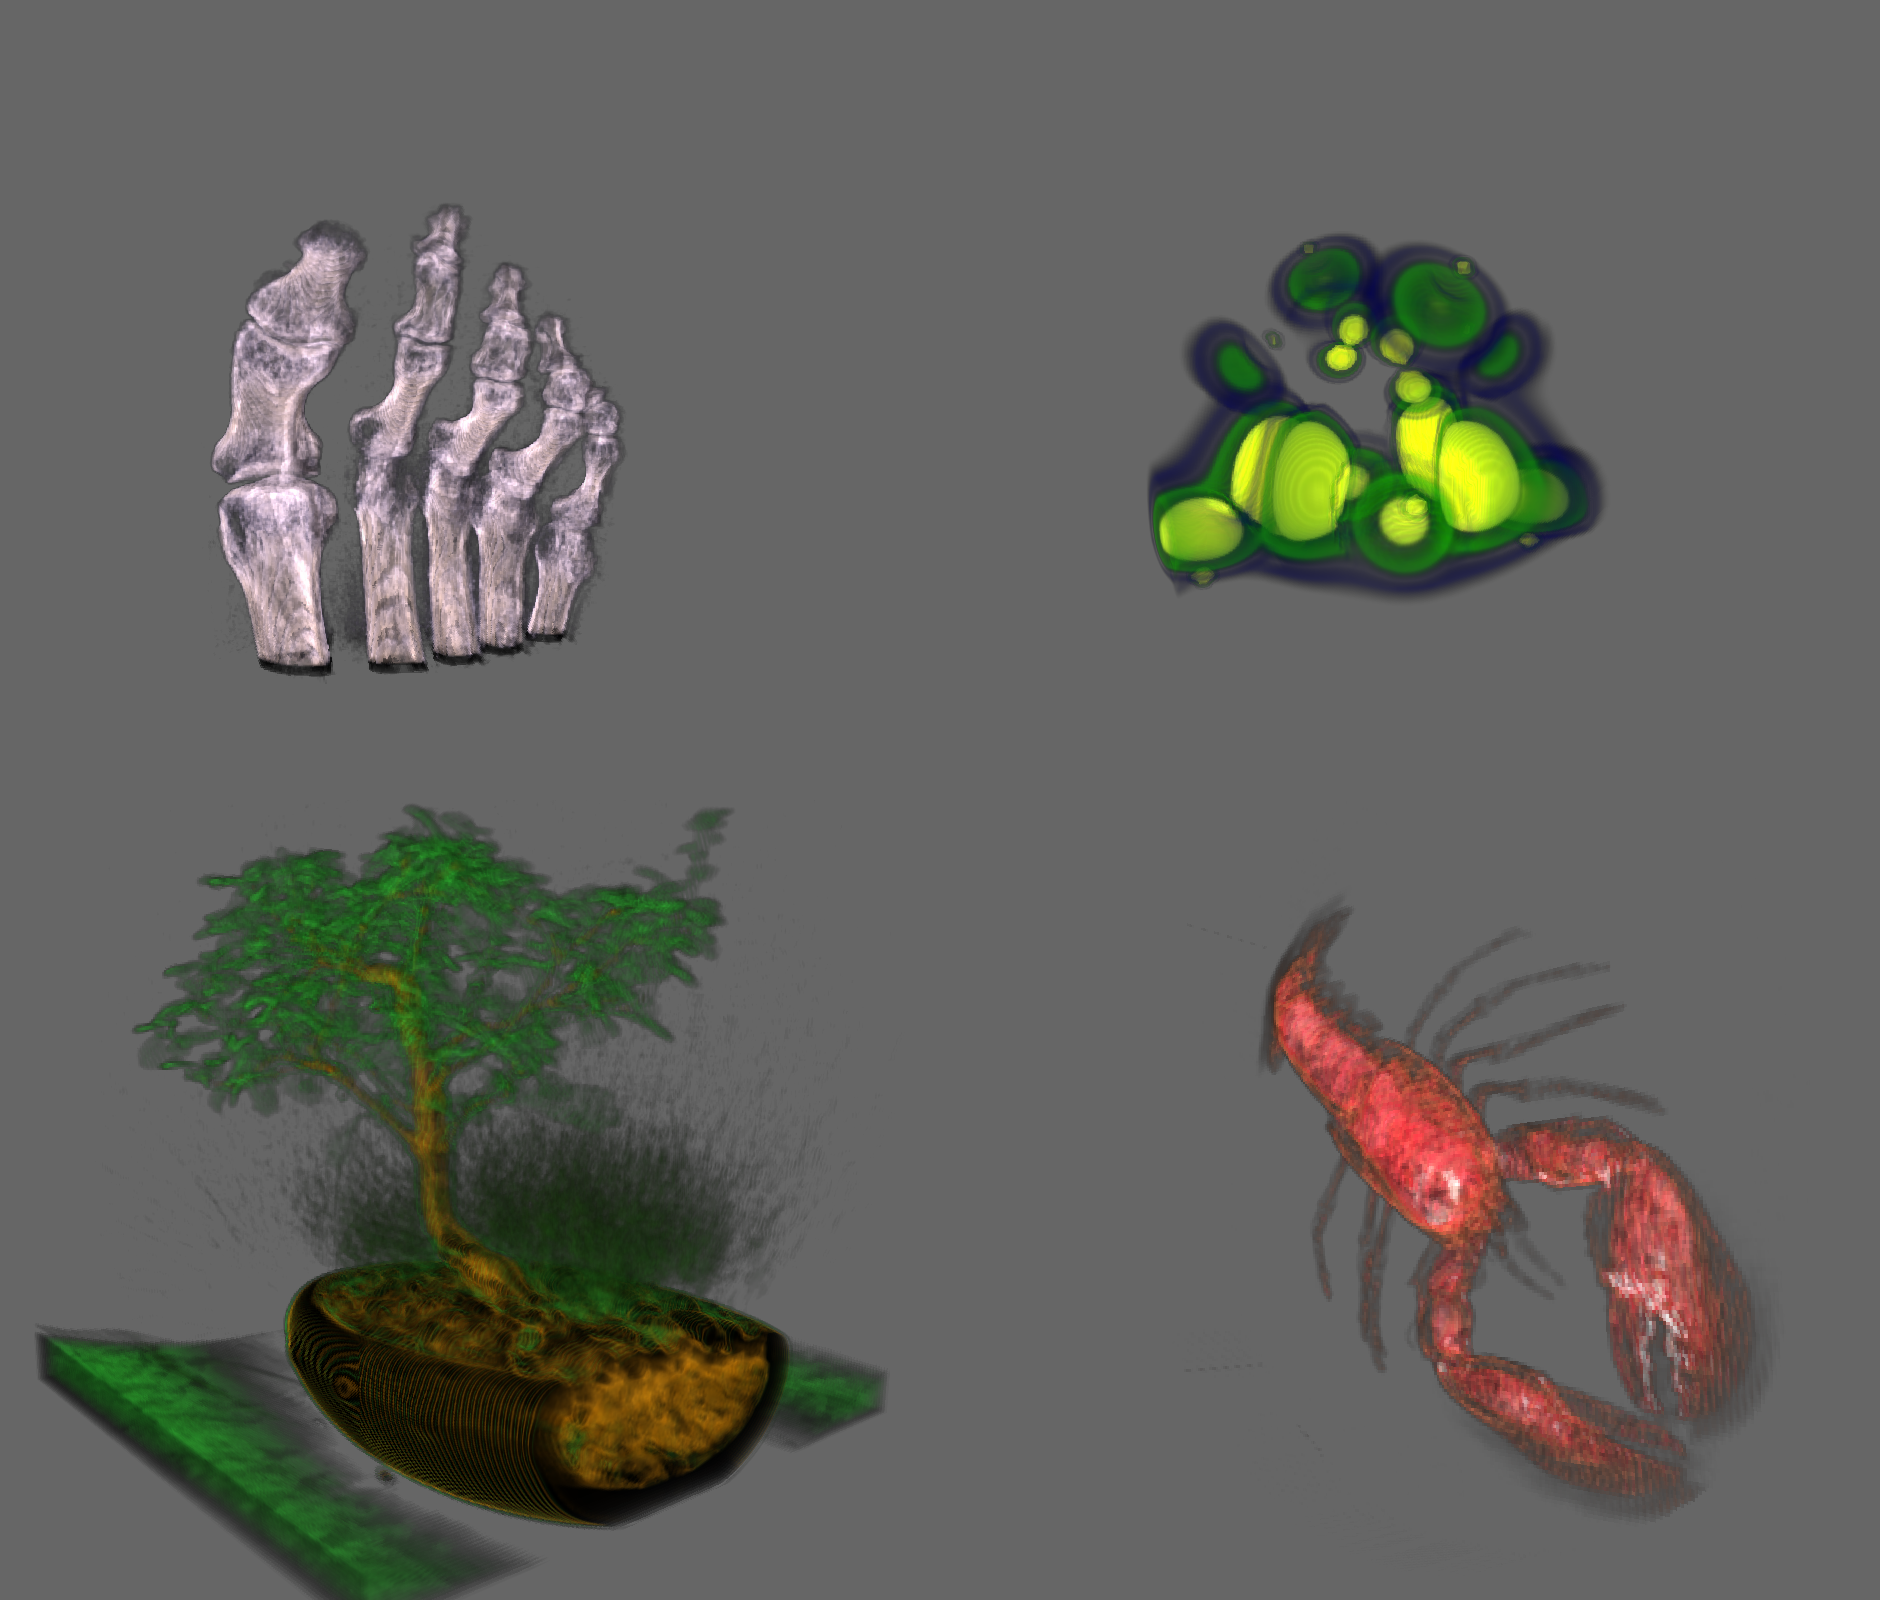
\includegraphics[height=11.5cm]{compare_3.png}
\caption{Apšvietimo sustiprinimo filtras.}
\label{fig:compare_3}
\end{figure}

